\documentclass[../main-v1.tex]{subfiles}
\begin{document}
\chapter{Overview of Computing Model \hideme{McNab - draft}}
\label{ch:cm}

%%%%%%%%%%%%%%%%%%%%%%%%%%%%%%%%
\section{Introduction}\label{ch:cm:intro} %\hideme{Schellman/McNab -needed}}
% Need a proper name

%SURF -> FNAL -> off site storage -> processing -> analysis

%Simulation -> storage -> analysis




The current \dword{dune} global computing model is an organic extension of the Fermilab \dword{fife} computing model, used for smaller Intensity Frontier experiments, to the full global collaboration.  This effort  has relied heavily on global infrastructure such as \dune{osg} and the \dword{wlcg} and was successful for the first small scale \dword{proto} tests. However, it needs substantial enhancement to cope with the data and processing volumes anticipated.  In this chapter we describe the current situation and proposals for future improvements. 

\subsection{Global resources}

\dword{dune} is a global collaboration with contributions from institutions worldwide.  The large scale computing effort relies on multi-national contributions. The long term strategy for computing resources is for primary raw data storage to reside at the large host labs (CERN and FNAL) with computing resources such as disk and CPU largely contributed by collaborating countries.   CPU contributions are provided by a large number of sites worldwide while storage is concentrated at a few larger international sites. Table \ref{tab:coop:disk} shows the distribution of disk space pledges for 2021 and 2022 while Tables \ref{tab:coop:sites} and \ref{tab:coop:ussites}shows the sites contributing CPU resources. 



%This model builds on the highly successful tools developed by the WLCG and OSG for LHC computing.  As DUNE's needs are substantially smaller that those of the large LHC experiments we can be confident that the existing infrastructure can be incrementally augmented to meet DUNE's requirements. 

%\section{Current Global Computing Model}


\begin{dunetable}
[National Disk pledges]{llrr}{tab:coop:disk}
{Disk pledges in PB for 2021 and 2022.}
Country/Lab	&	Name	&	2021	&	2022	\\
FNAL	&	FNAL	&	2.2	&	7.6	\\
CERN	&	CCERN	&	2.2	&	1.6	\\
BNL	&	BNL	&	0.5	&	0.5	\\
UK	&	GridPP	&	4.0	&	4.0	\\
FR	&	CC-IN2P3	&	0.5	&	0.5	\\
ES	&	PIC Tier-1	&	0.5	&	0.72	\\
NL	&	NL/LHC Tier-1	&	1.9	&	1.8	\\
CZ	&	CZ-Prague-T2	&	0.3	&	1.0	\\
%BR	&	CBPF	&	0	&		\\
IN	&	TIFR	&	0.75&	0.75\\
RU	&	JINR	&	-	&	0.5	\\
\hline
Total pledge	&		&	12.85	&	18.97	\\
\end{dunetable}

%\tiny
\begin{dunetable}
[List of DUNE Compute Sites]
{l l r l}{tab:coop:sites}
{List of non-US international DUNE compute sites as of December 2021.  Sites with substantial rucio controlled disk are noted.}
Site name	&	RC Site	&	Disk	&	Country	\\
\hline
BR\_CBPF	&	BR\_CBPF	&		&	Brazil\\
BR\_UNICAMP	&BR\_UNICAMP	&		&	Brazil\\
CA\_Victoria	&	CA\_Victoria	&		&	Canada\\
CERN	&	CERN-PROD	&	Yes	&	Switzerland\\
CH\_UNIBE-LHEP	&	UNIBE-LHEP	&		&	Switzerland\\
CZ\_FZU	&	FZU	&	Yes	&	Czechia\\
ES\_CIEMAT	&	CIEMAT-LCG2	&		&	Spain\\
ES\_PIC	&	pic	&	Yes	&	Spain\\
FR\_CCIN2P3	&	IN2P3-CC	&	Yes	&	France\\
IN\_TIFR	&	IN\_TIFR	&	Yes	&	India\\
NL\_NIKHEF	&	NIKHEF-ELPROD	&		&	Netherlands\\
NL\_SURFsara	&	SURFsara	&	Yes	&	Netherlands\\
RU\_JINR	&	JINR\_CONDOR\_CE	&	Yes	&	Russian Federation\\
UK\_Bristol	&	UKI-SOUTHGRID-BRIS-HEP	&		&	United Kingdom\\
UK\_Brunel	&	UKI-LT2-Brunel	&		&	United Kingdom\\
UK\_Edinburgh	&	UKI-SCOTGRID-ECDF	&		&	United Kingdom\\
UK\_Imperial	&	UKI-LT2-IC-HEP	&		&	United Kingdom\\
UK\_Lancaster	&	UKI-NORTHGRID-LANCS-HEP	&	Yes	&	United Kingdom\\
UK\_Liverpool	&	UKI-NORTHGRID-LIV-HEP	&		&	United Kingdom\\
UK\_Manchester	&	UKI-NORTHGRID-MAN-HEP	&	Yes	&	United Kingdom\\
UK\_Oxford	&	UKI-SOUTHGRID-OX-HEP	&		&	United Kingdom\\
UK\_QMUL	&	UKI-LT2-QMUL	&	Yes	&	United Kingdom\\
UK\_RAL-PPD	&	UKI-SOUTHGRID-RALPP	&		&	United Kingdom\\
UK\_RAL-Tier1	&	RAL-LCG2	&	Yes	&	United Kingdom\\
UK\_Sheffield	&	UKI-NORTHGRID-SHEF-HEP	&		&	United Kingdom\\

\end{dunetable}
\begin{dunetable}
[List of US DUNE Compute Sites]
{l l r l}{tab:coop:ussites}
{List of US DUNE compute sites as of December 2021.  Sites with substantial rucio controlled disk are noted.}
US\_UConn-HPC	&	UConn-HPC	&		&	United States\\
US\_BNL	&	BNL-SDCC-CE01	&	Yes	&	United States\\
US\_Caltech	&	CIT\_CMS\_T2	&		&	United States\\
US\_Clemson	&	Clemson-Palmetto	&		&	United States\\
US\_Colorado	&	UColorado\_HEP	&		&	United States\\
US\_Florida	&	UFlorida-HPC	&		&	United States\\
US\_FNAL	&	GPGrid	&	Yes	&	United States\\
US\_KSU	&	BEOCAT-SLATE	&		&	United States\\
US\_Lincoln	&	Rhino	&		&	United States\\
US\_Michigan	&	AGLT2	&		&	United States\\
US\_MIT	&	MIT\_CMS	&		&	United States\\
US\_MWT2	&	MWT2	&		&	United States\\
US\_Nebraska	&	Nebraska	&		&	United States\\
US\_NERSC & NERSC &   & United States\\
US\_NMSU-DISCOVERY	&	SLATE\_US\_NMSU\_DISCOVERY	&		&	United States\\
US\_NotreDame	&	NWICG\_NDCMS	&		&	United States\\
US\_Omaha	&	Crane	&		&	United States\\
US\_PuertoRico	&	uprm-cms	&		&	United States\\
US\_SU-ITS	&	SU-ITS-CE2	&		&	United States\\
US\_UChicago	&	MWT2	&		&	United States\\
US\_UCSD	&	UCSDT2	&		&	United States\\
US\_Wisconsin	&	GLOW	&		&	United States\\
US\_WSU	&	WSU - GRID\_ce2	&		&	United States\\
\end{dunetable}
%\todo{Add diagrams}

\section{Current performance}. 

\dword{dune} have performed multiple simulation and reconstruction passes on the \dword{pdsp} data and are running significant simulation campaigns for the \dword{fd} and \dword{nd} design and physics studies. The \dword{poms} and \dword{sam} described in Chapters \ref{ch:datamgmt} and \ref{ch:flow}, are highly instrumented and allow assessments of the performance of the global computing system in near-real time.  There are four major data/cpu access patterns.
\begin{itemize}
    \item Simulation requires little input (mainly beam flux files and photon libraries),  has a large memory footprint, uses significant CPU resources and writes back a few large files.
    \item Data reconstruction reads in large files, has an intermediate memory footprint and uses $\sim$ 10 sec/MB of input data.  
    \item Data reduction reads the reconstructed data and produces small tuple outputs for further analysis.  Reduction uses $\sim 0.1$ sec/MB of input data and is generally IO limited.
    \item Data analysis consists of repeated access to smaller tuple outputs for calibration and parameter estimation.
\end{itemize}

Each of these use cases is best suited for a different combination of data/cpu resources and the global compute model should be able to allocate resources appropriately.  

We have used the \dword{sam} instrumentation to measure the \dword{xrootd} streaming performance for disk/cpu location combinations. 

\begin{dunefigure}
[Streaming speeds for reconstruction]
{fig:recospeed} 
{Streaming speeds for reconstruction jobs running at different locations. Raw data are stored at CERN and Fermilab.  The histograms show the log10 of the inferred streaming rate (wall time/file size) for reconstruction jobs running at selected sites with different data sources.}
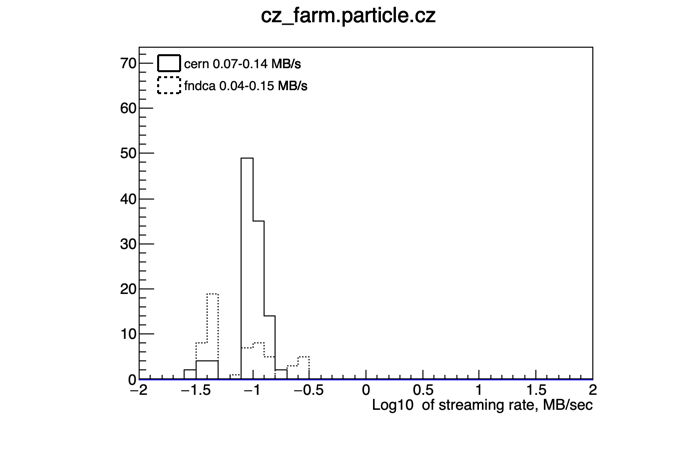
\includegraphics[width=0.45 \textwidth]{graphics/Workflow/dune_slow_2021_01_01_2021_04_30_0_cz_farm.particle.cz.png}
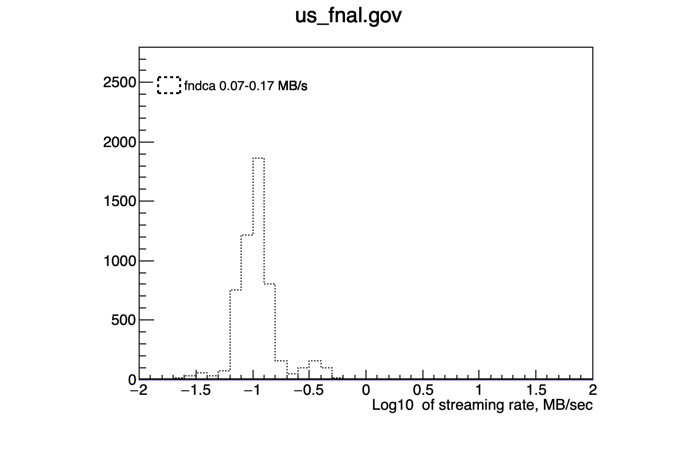
\includegraphics[width=0.45 \textwidth]{graphics/Workflow/dune_slow_2021_01_01_2021_04_30_0_us_fnal.gov.png}
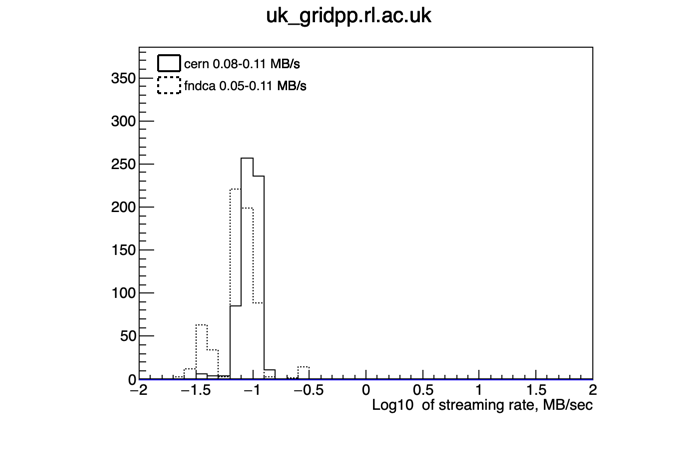
\includegraphics[width=0.45 \textwidth]{graphics/Workflow/dune_slow_2021_01_01_2021_04_30_0_uk_gridpp.rl.ac.uk.png}
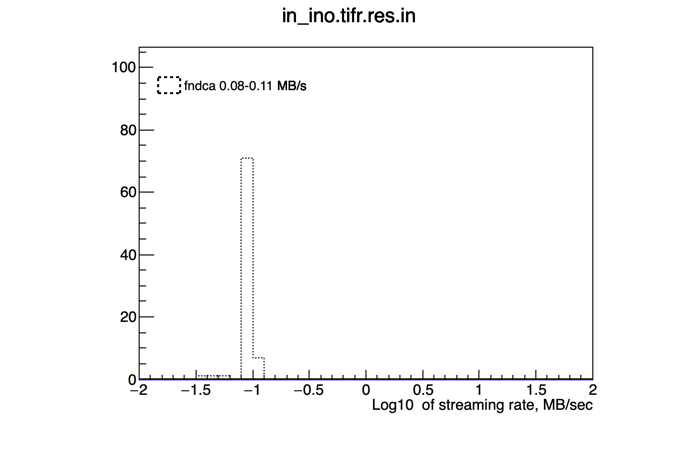
\includegraphics[width=0.45 \textwidth]{graphics/Workflow/dune_slow_2021_01_01_2021_04_30_0_in_ino.tifr.res.in.png}
\end{dunefigure}
%\todo{Get better figure}


\begin{dunefigure}
[Streaming speeds for tuple creation]
{fig:tuplespeed} 
{Streaming speeds for tuple creation jobs running at selected locations during a test in early January 2022. Reconstructed simulation files were located at sites in the UK and at Fermilab.  The histograms show the log10 of the inferred streaming rate (wall time/file size) for tuple creation jobs running at selected sites with different data sources.}
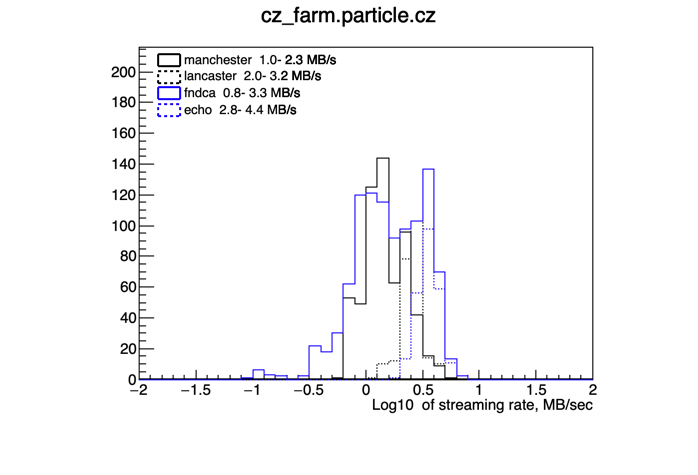
\includegraphics[width=0.45 \textwidth]{graphics/Workflow/dune_fast_2022_01_01_2022_01_07_0_cz_farm.particle.cz.png}
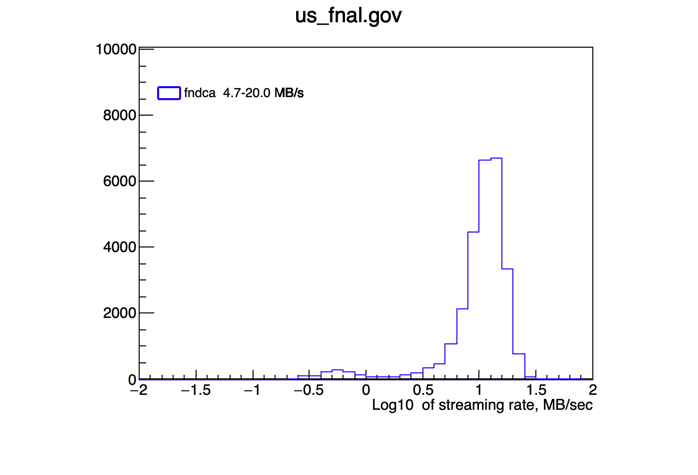
\includegraphics[width=0.45 \textwidth]{graphics/Workflow/dune_fast_2022_01_01_2022_01_07_0_us_fnal.gov.png}
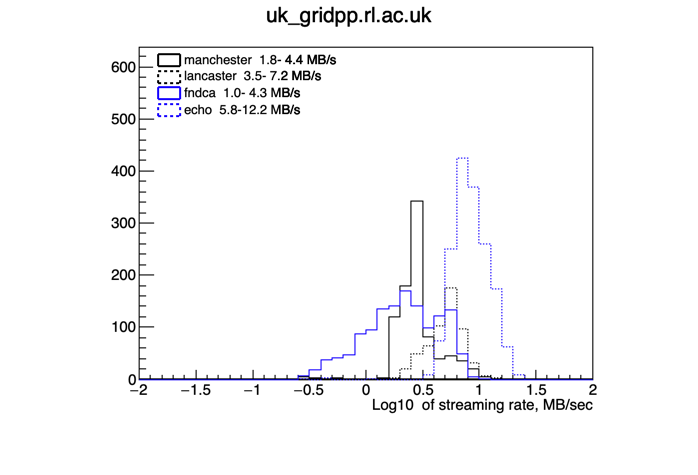
\includegraphics[width=0.45 \textwidth]{graphics/Workflow/dune_fast_2022_01_01_2022_01_07_0_uk_gridpp.rl.ac.uk.png}
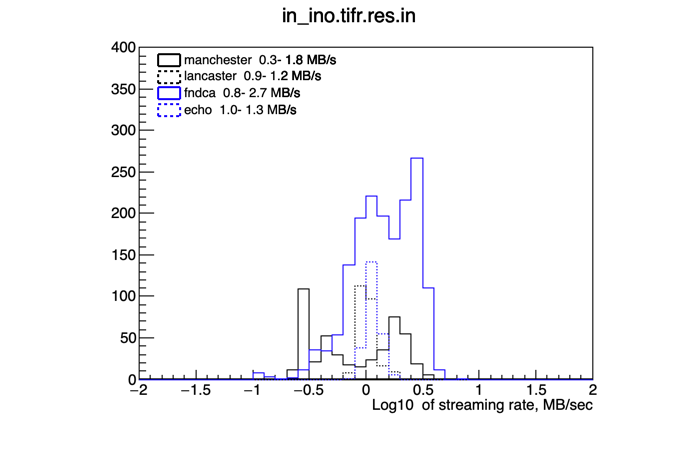
\includegraphics[width=0.45 \textwidth]{graphics/Workflow/dune_fast_2022_01_01_2022_01_07_0_in_ino.tifr.res.in.png}
\end{dunefigure}
%\todo{Get better figure}

\begin{dunefigure}
[Streaming speeds for tuple creation]
{fig:tuplespeedsummary} 
{Streaming speeds for tuple creation jobs running at multiple locations during a test in early January 2022. Reconstructed simulation was stored at sites in the UK and at Fermilab.  The average estimated streaming rates are plotted as a function of disk location (x-axis) and compute site (y-axis). Jobs in the US were required to use Fermilab disk but international sites were tested with multiple samples.}
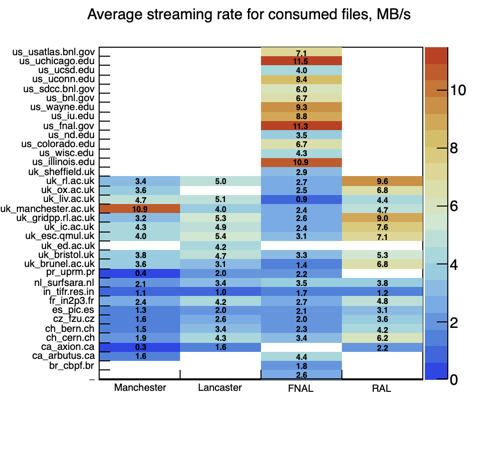
\includegraphics[width=0.8 \textwidth]{graphics/Workflow/fastRates.png}
\end{dunefigure}

\subsection{Implications for data and processing placement}

The current study indicates that for CPU dominated applications, notably reconstruction of raw data and simulation, the relative location of CPU resources is not critical. Wall time/MB   is similar regardless of location. 

For IO dominated applications, proximity to the data is important.  Here there is a tradeoff between the availability of resources and the efficiency with which they can be used. Inter-US processing, especially for locations near the national laboratories, is highly efficient, as is processing within the UK.  However, efficiency falls of as the CPU and disk become more separated.  

We have the monitoring tools to provide a workflow management system with the information it needs to do optimal placement of data and jobs to maximize efficiency. However our existing data management and workflow tools are not able to take full advantage of this information.  This motivates development of an improved workflow model described below and in Chapter \ref{ch:wkflow}.

\section{Sites and Services \hideme{McNab - draft}}
\label{sec:cm:sites_and_services}  %% fix label according to section

% Some of this should goes to the Site Resources chapter 
% References to APIs and specific technologies
% perhaps even the definitions types of center and site too

The large LHC experiments have historically relied on a tiered structure, with national Tier-1 centers serving regional Tier-2 and Tier-3 centers.  The DUNE model builds on the emergence of faster networks to move to  a service-oriented model, where sites provide services, disk, CPU, real memory/core and archival tape, and projects are  distributed to them based on their capabilities and available networking.  For example, a site with large CPU and memory/core but slower networking would be ideal for simulation while small memory/core and fast access to large local disk stores would be ideal for high level data analysis.  This model will require a high level view of data locations and job placement with continual monitoring for bottlenecks but allows new sites to contribute in an optimal way. 

This section sets out our ``Sites and Services'' model for using sites for DUNE computing tasks, including sites that participate in OSG or WLCG more generally. Since our requirements are not the same as the LHC experiments, this necessitates a distinct naming scheme to WLCG and ways of mapping our scheme onto the WLCG tier model.

At this stage, DUNE has chosen to express its requirements in terms of services provided by sites. Each site provides networking plus one or more approved DUNE services, which satisfy DUNE's minimum requirements for the service in terms of capacity, quality, and interfaces.

This model allows us to avoid making assumptions about how sites and federations of sites will be organised in the future, as the community evolves away from the strict WLCG tiers model towards DOMA and concepts like data lakes: instead we express our requirements in terms of the services we interact with.

DUNE expects to be able to access services using broadly the same set of APIs as WLCG (eg HTCondor-CE and xroot) and by using common cloud APIs (eg OpenStack and S3). For this reason, sites may be operated using conventional grid technologies, on-premises cloud systems, or commercial cloud services.

Nevertheless, sites do appear in the DUNE computing model, as the atomic unit for operations activity. For example, staff at a site can receive and process tickets, may have a representative at an operations meeting with the technical knowledge to comment on issues as they arise.

In terms of workflows and data management, DUNE does not impose or require any hierarchy or grouping of sites, and assumes that, in general, data may flow between services at any two sites. Having said that, DUNE expects to use network proximity and bandwidth information to guide the efficient transfers of data between services. 

\section{Sites, Federations, and Countries\hideme{McNab - draft}}
\label{sec:cm:federations}

As well as sites, there are two more administrative concepts: federations and countries.

Federations are borrowed from WCLG and represent one or more sites which together pledge a particular amount of capacity to DUNE, and enter their pledges into a system like CRIC. Sites may choose to organise themselves this way as it allows more flexibility in how pleges are met against a background of planned upgrades at sites, unplanned outages etc. 

Countries are represented directly or indirectly at the DUNE Computing Contributions Board, and consist of one or more federations. Broadly, countries map to funding bodies and are the basis of comparison between level of contribution to computing capacity and number of DUNE members.




\section{Types of service\hideme{McNab - draft}}
\label{sec:cm:types_of_service}

We envisage 5 classes of service, on which we will put requirements and request capacity.

\begin{itemize}
    \item Network
    \item DUNE Computing Element
    \item Data Cache
    \item DUNE Storage Element
    \item DUNE Data Archive
\end{itemize}

\subsection{Network\hideme{McNab - draft}}
\label{sec:cm:network}

Networking is needed at all sites, with basic requirements including IPv4 and IPv6.
All sites should be connected to the wide area network, typically via their NREN, with sufficient capacity to handle the data I/O commensurate with their fraction of the workload. In practice this means at least 40 Gbit/s for major sites with large amounts of storage (with 100 Gbit/s becoming the normal expectation for a shared site such as a WLCG Tier-1) and at least 20 Gbit/s for smaller CPU only sites (but with 40-100 Gbit/s becoming the norm in shared sites).
Other DUNE approved services may impose further requirements in terms of network capacity which they require,

\subsection{DUNE Computing Element\hideme{McNab - draft}}
\label{sec:cm:dce}

A DUNE Computing Element is a service which gives access to jobs consuming CPU to perform computation. To the operational overhead in working with each site, DUNE will require a minimum standards for

\begin{itemize}
    \item The support level, in terms of whether tickets will be acted 24/7 or only during working hours
    \item The total number of logical processors across the service
    \item The interface used to submit jobs or create virtual machines
    \item Operating system version for grid capacity
    \item Memory and scratch disk per processor
    \item Incoming and outgoing network capacity per processor
    \item Suitable access to a DUNE Storage Element or Data Cache, which allows data intensive jobs to execute without an unacceptably low CPU efficiency
\end{itemize}

We envisage three subclasses within the computing element services aimed at centrally managed data processing, at user or working group data analysis, and at detector simulation. These subclasses have different requirements for network access, and in the case of data analysis, for support level.

\subsection{Data Cache\hideme{McNab - draft}}
\label{sec:cm:data_cache}

Suitable networking. Sufficient nearby DUNE Compute Element capacity to be useful. Not managed by DUNE systems. ``Transparent''. Data loss is equivalent to jobs dying, so a transient which DUNE systems will recover from.

\subsection{DUNE Storage Element\hideme{McNab - draft}}
\label{sec:cm:dse}

The concept of a DUNE Storage Element mirrors that of a DUNE Compute Element. It must be of sufficient capacity, measured in hundreds of TB or PB, for the operational overheard to be worthwhile. It must have a suitable support level, in terms of whether tickets will be acted 24/7 or only during working hours. There must be enough inbound and outbound networking capacity for global data placement operations, and for jobs to write data there or to consume the data already present. In particular, there must be a minimum amount of DUNE Compute Element capacity available nearby, on which DUNE jobs can access the storage service without an unacceptably low CPU efficiency. 

This formulation allows conventional grid sites with CPU and disk storage mixed together in adjacent racks, but also novel regional architectures such as data lakes in which there is sufficient network capacity to link CPU and storage at different locations. At this stage of the project, DUNE does not want to prejudge what will be available at the start of data taking, and does not want to discourage the exploration of new and more efficient ways of providing resources.

\subsection{DUNE Data Archive\hideme{McNab - needs work}}

Networking. Cache? Support level? Tape without saying only tape forever.

%The host laboratory is the most important center and during DUNE data %taking will be FNAL. During protoDUNE data taking, both FNAL and CERN %have host laboratory roles. A host laboratory runs central services %for DUNE, makes the largest single contribution in disk and CPU, and %acts as an archive center and user center. This broadly corresponds %to the WLCG Tier-0 concept. 
%
%Archive centers fulfill DUNE’s requirement to have two copies of raw %data on tape (or other archival-quality storage systems), including %one not at the Host Laboratory. It is not essential that archive %centers also have significant amounts of disk and CPU available to %DUNE as they may only be needed for disaster recovery and for %recovering individual lost files. Amongst WLCG sites, archive centers %would be based on the tape archives of Tier-1s, and the concept maps %directly to the DOMA idea of an archive center where disk storage and %CPU may be absent.
%
%Disk centers provide storage managed by DUNE, along with significant %amounts of CPU, and satisfy DUNE’s requirements for the ratio of CPU %to disk, the bandwidth between CPU and disk, and the bandwidth to and %from other participating centers. DUNE does not require 24/7 on call %support for disk centers, but may use the declared support level when %deciding where to place data and where to direct workflows. Disk %centers correspond to WLCG Tier-1 sites or Tier-2 sites with disk, %and to DOMA Data and Compute Centers.
%
%Compute centers provide only CPU capacity, scratch disk associated %with jobs running on worker nodes for the duration of jobs, and %possibly transparent caching (eg Xcache). That is, they do not %provide storage which is managed by DUNE. They do however satisfy %DUNE’s requirements for bandwidth to and from other participating %centers. Compute centers correspond to WLCG Tier-2 sites without %disk, and to DOMA compute centers. 
%
%User centers are used for end user analysis, by people submitting %jobs and managing workflows, and may need to download or stream a %limited amount of data directly from disk centers.


\section{Requirements for computing services \hideme{McNab - needs work}}

What we need DUNE services to be able to do, to do the above.

\todo{consider both cases of data to job and job to data - discuss current issues but be vague about the future}

%%%%%%%%%%% notes from 10-29

% Define a minimal "CPU-only" service

% Define a DUNE-managed disk service - how many TB min - requires support. 

% Define a tape service

% Mention possible need for cache for 

%(How do they get the code? cvmfs or container.  

\todo{Andrew compares the use case footprint table into a sites comparison}
\end{document}